% to render
% pdflatex [ filename ] && pdflatex [ filename ]

\documentclass{article}
% \documentclass[twocolumn]{article}


\usepackage{graphicx}
\usepackage{amsmath, amsthm, amssymb}
\usepackage{parskip}

% block code
\usepackage{alltt}

% set margins
\usepackage[margin = 1in]{geometry}
\setlength{\parindent}{1cm}

\usepackage{setspace}
% for double spacing the entire document
% \doublespacing
\singlespacing

% fancier captions
\usepackage{caption}
\captionsetup[figure]{font = small, labelfont = small}

%% imported packages
\usepackage{paralist}

% reference tables and figures, in the style of eqref
\newcommand{\figref}[1]{Fig. (\ref{#1})}
\newcommand{\tabref}[1]{Table (\ref{#1})}

% stylistic shortenings
\newcommand{\ti}[1]{\emph{#1}}
\newcommand{\tb}[1]{\textbf{#1}}
\newcommand{\cpart}[1]{\newblock{\LARGE {\\\\#1}}}
\renewcommand{\arraystretch}{1.3}

% comments that should be hidden
\newcommand{\comment}[1]{}

% note syntax
\newcommand{\note}[1]{\newblock{\small [ \ti{\tb{#1}} ]}}
% hide notes
% \newcommand{\note}[1]{\comment{#1}}

% inline code
\newcommand{\code}[1]{\texttt{$\text{#1}$}}

% vector stylization
\newcommand{\vect}[1]{\boldsymbol{#1}}
% \newcommand{\vect}[1]{\vec{#1}}

\begin{document}
% small text
% \small

\title{\tb{Lock Implementations}}
\author{Minke Zhang\hspace*{-\tabcolsep}}
\date{\today}

% make title
\begingroup
\let\center\flushright
\let\endcenter\endflushright
\maketitle
\endgroup

\section{Modules}

\cpart{Locks}

We wish to abstract away the specifics of the lock interface so that at lock invocation, we do not need to worry about how to handle each type of lock. As such, we 
will allow a lock struct to deal with the complexities of each lock, and to provide a standard interface for the experiments.

\begin{alltt}
struct lock_t \{
  int type;             // the type of lock being used
  int status;           // a copy of the lock status
  void *l;              // the lock
\} lock;

lock *init_lock(int type);
void lock(lock *l) \{
  switch(l->type) \{
    ...
  \}
  l->status = 1;
\}

int try_lock(lock *l) \{
  return(status);
\}

void unlock(lock *l) \{
  switch(l->type) \{
    ...
  \}
  l->status = 0;
\}
\end{alltt}

\cpart{Experiment Interfaces}

What follows is the expected interface for experiments-- the hope being that if all else is sufficient, we will simply alter the given variables and

\begin{alltt}
int time_counter_serial(int M);                         // returns the counter value at
                                                        //   M seconds
int time_counter_parallel(int M, int n, int L);         // returns the counter value at
                                                        //   M seconds, with n threads
                                                        //   and lock type L

float work_counter_serial(int B);                       // returns the time taken for
                                                        //   the counter to reach B
float work_counter_parallel(int B, int n, int L);       // returns the time taken for
                                                        //   the counter to reach B,
                                                        //   with n threads and lock
                                                        //   type L

void packet_serial(int M, int n, long W, int            // same as the serial version
  uniform_flag, short experiment_number);               //   of the last project, but
                                                        //   without specifying T
void packet_parallel(int M, int n, long W, int          // parallel version, with (non)-
  uniform_flag, short experiment_number, int D,         //   locking dequeues and load
  int L, int S);                                        //   balancing strategy S
\end{alltt}

\section{Hypotheses}

TaS, exponential, mutex, anderson, CLH

\cpart{Idle Overhead}

We would expect that the overhead generated by the TAS and backoff lock will not significantly slow down the parallel counter-- the length of the uncontested path 
is a simple straight walk through the \code{lock()} function, whereas the queue-based locks will require memorry allocation per lock call, and as such, should incur 
a higher overhead penalty. The POSIX lock implementation is, as per StackOverflow (http://bit.ly/MHnDdX), a userspace increment-and-test implementation, which is 
hardware instruction based; as such, we would expect the performance of the POSIX implemenation to lie closer to TAS at $n = 1$ than to the queue-based locks.

\cpart{Lock Scaling}

As was mentioned in class, we would expect that the TAS and backoff locks to behave rather poorly under heavy contention, whereas the queue-based locks are much 
better at adjusting to the heavier congestion, as the queue-based locks avoid in large part the expensive cache misses which occur for conventional locks.

\cpart{Fairness}

We would expect that the TAS to have a much higher deviation than the queue-based locks, due to possibilities of starvation of certain threads in cases of heavy 
contention, whereas the queue-based locks should have a small deviation due to the way in which lock requests are being made.

\cpart{Packet Overhead}

We believe there will be more overhead generated due to the homequeue lock implementation-- because the nature of locks, we are serializing a process which was 
before perfectly fine being modified concurrently. Thus, we would expect the worker rate to be lower for implementations of the firewall utilizing locks than using 
the lock-free queue. Moreover, we would expect that the relative overhead between lock implementations to mirror that of the \tb{idle overhead}.

\cpart{Packet Scaling}

We do not believe there to be a significant speedup while using locks in the uniform packet case-- the use of locks for the firewall is to provide a way for 
multiple threads to call \code{dequeue()} on a queue simultaneously. This is only useful for the case of load-balancing, which will only be a major consideration in 
the exponentially distributed packet case. We will therefore expect the \ti{awesome} strategy to emphasize high number of threads using the queue-based lock, and 
with some work-stealing scheduling implemented.

\section{Data \& Analysis}

\cpart{Idle Overhead}

\begin{table}
\begin{center}
	\begin{tabular}{ r | c c }
		lock		&	$R_T$	&	$R_W$	\\
		\hline
		test and set	&	0.108	&	0.020	\\
		backoff		&	0.100	&	0.021	\\
		pthread mutex	&	0.132	&	0.025	\\
		Anderson	&	0.221	&	0.045	\\
		CLS		&	0.200	&	0.044	\\
	\end{tabular}
\end{center}
\caption{Performance ratios for the parallel time-limit based counter ($R_T$) and parallel work-limit based counter ($R_W$) for a variety of lock schemas, as compared to the serial counters.}
\label{idle_table}
\end{table}

\cpart{Lock Scaling}

\begin{figure}
\begin{center}
	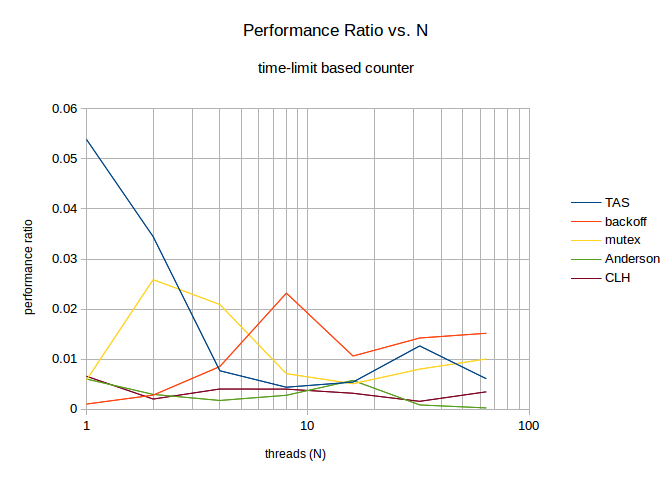
\includegraphics[scale=.8]{counter_3.png}
	\caption{Performance ratios for the parallel time-limit based counter for different lock schemas, as compared to the serial implementation.}
	\label{counter_3}
\end{center}
\end{figure}

\begin{figure}
\begin{center}
	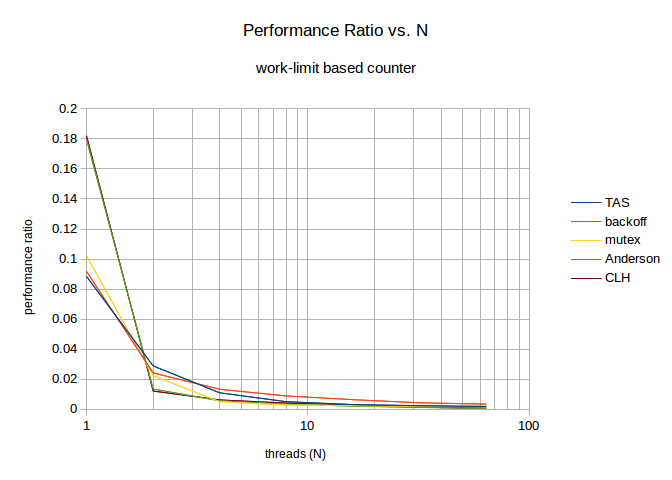
\includegraphics[scale=.8]{counter_4.png}
	\caption{Performance ratios for the parallel work-limit based counter for different lock schemas, as compared to the serial implementation.}
	\label{counter_4}
\end{center}
\end{figure}

\cpart{Fairness}

\begin{figure}
\begin{center}
	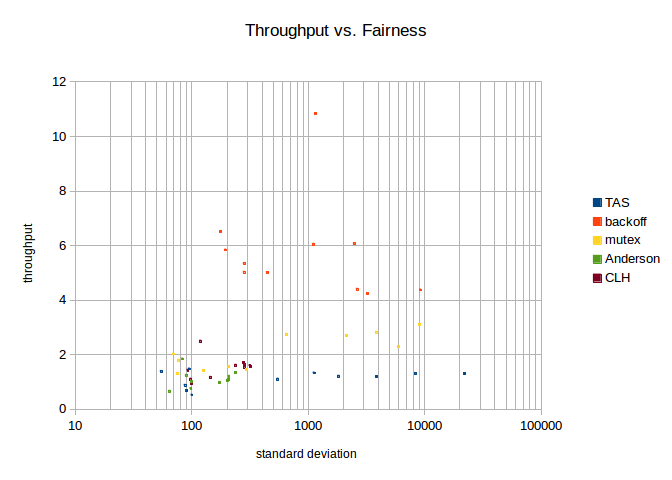
\includegraphics[scale=.8]{counter_5.png}
	\caption{Throughput as a function of the standard deviation of worker contributions in the time-limit based counter.}
	\label{counter_5}
\end{center}
\end{figure}

\cpart{Packet Overhead}

\begin{figure}
\begin{center}
	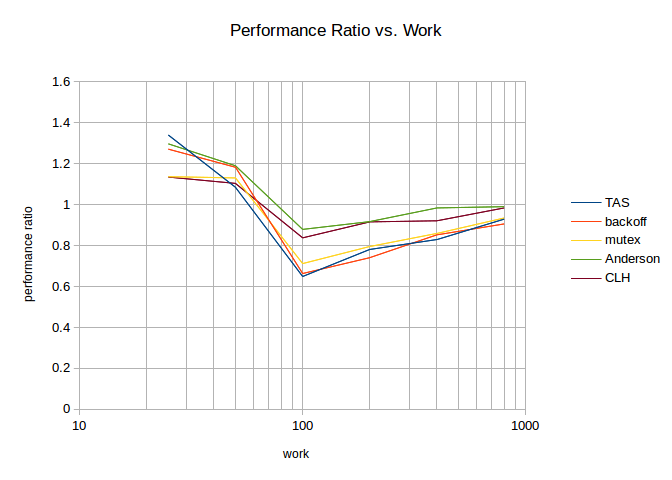
\includegraphics[scale=.8]{packet_1.png}
	\caption{Performance ratios for the \code{HomeQueue} firewall as compared to the \code{LockFree} implementation, as a function of the work involved per packet.}
	\label{packet_1}
\end{center}
\end{figure}

\cpart{Packet Scaling}

\begin{figure}
\begin{center}
	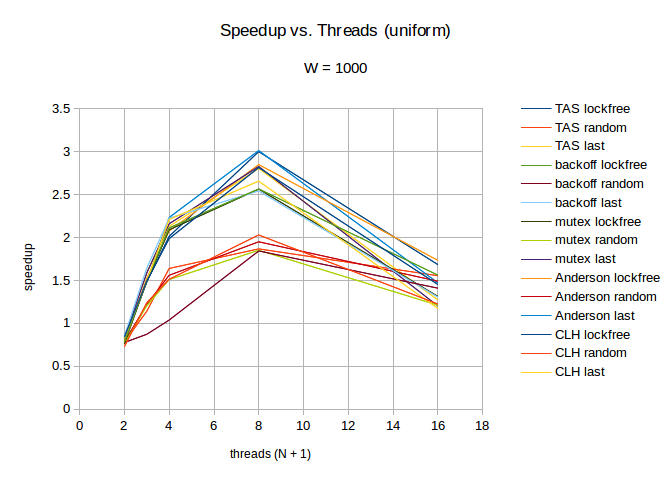
\includegraphics[scale=.8]{packet_2_1000.png}
	\caption{Performance ratios for parallel firewall, with uniform packet distribution at mean work $W = 1000$.}
	\label{packet_2_1000}
\end{center}
\end{figure}

\begin{figure}
\begin{center}
	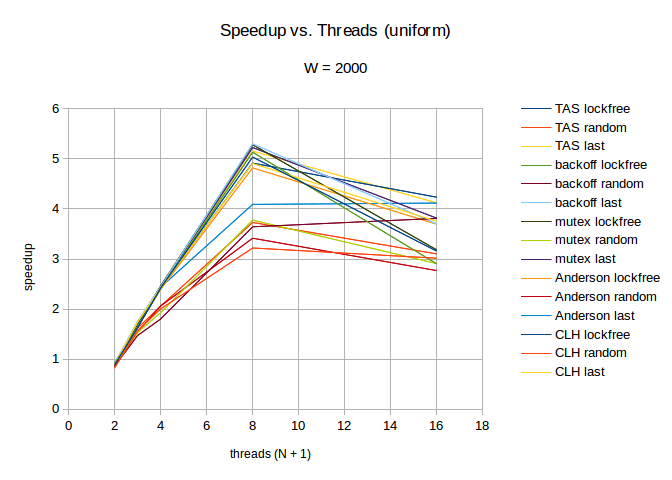
\includegraphics[scale=.8]{packet_2_2000.png}
	\caption{Performance ratios for parallel firewall, with uniform packet distribution at mean work $W = 2000$.}
	\label{packet_2_2000}
\end{center}
\end{figure}

\begin{figure}
\begin{center}
	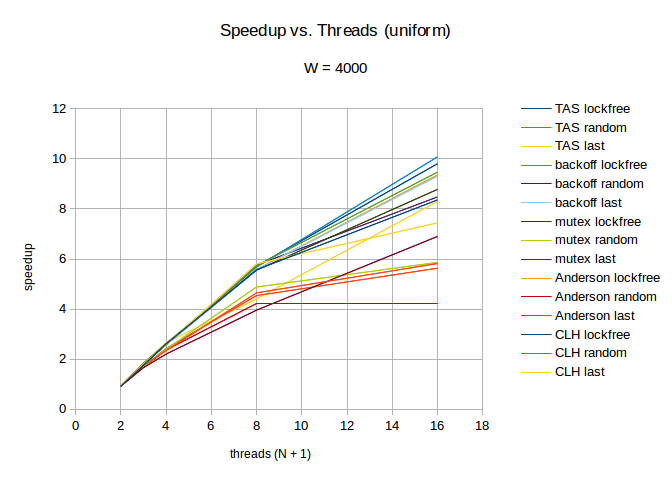
\includegraphics[scale=.8]{packet_2_4000.png}
	\caption{Performance ratios for parallel firewall, with uniform packet distribution at mean work $W = 4000$.}
	\label{packet_2_4000}
\end{center}
\end{figure}

\begin{figure}
\begin{center}
	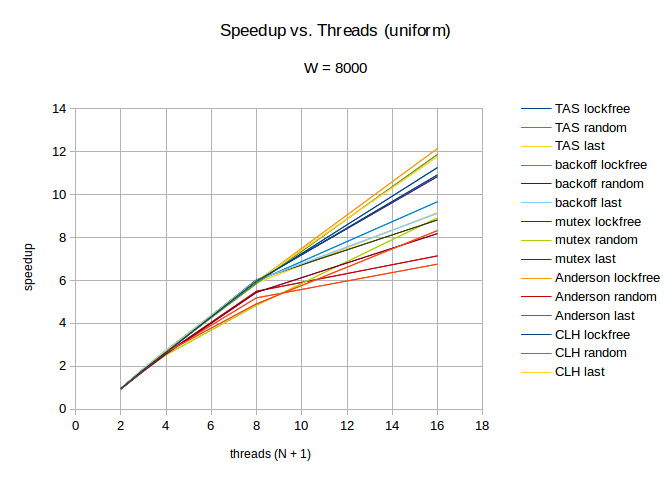
\includegraphics[scale=.8]{packet_2_8000.png}
	\caption{Performance ratios for parallel firewall, with uniform packet distribution at mean work $W = 8000$.}
	\label{packet_2_8000}
\end{center}
\end{figure}

%----------------------------------------------

\begin{figure}
\begin{center}
	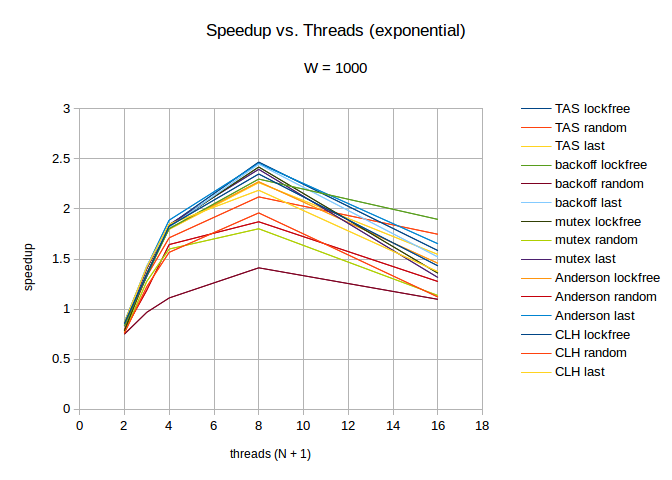
\includegraphics[scale=.8]{packet_3_1000.png}
	\caption{Performance ratios for parallel firewall, with exponential packet distribution at mean work $W = 1000$.}
	\label{packet_3_1000}
\end{center}
\end{figure}

\begin{figure}
\begin{center}
	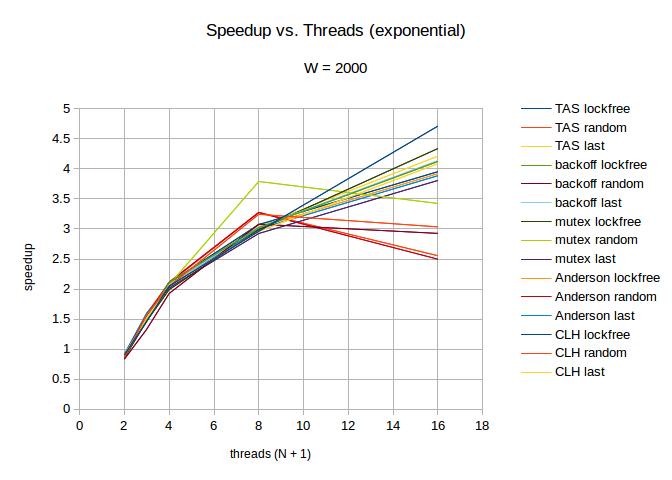
\includegraphics[scale=.8]{packet_3_2000.png}
	\caption{Performance ratios for parallel firewall, with exponential packet distribution at mean work $W = 2000$.}
	\label{packet_3_2000}
\end{center}
\end{figure}

\begin{figure}
\begin{center}
	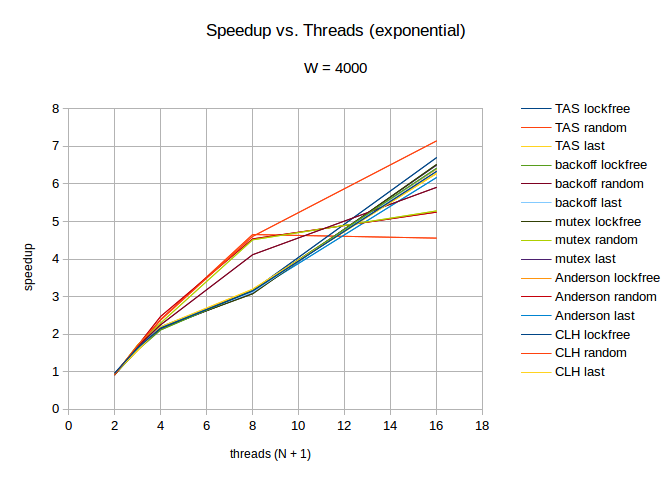
\includegraphics[scale=.8]{packet_3_4000.png}
	\caption{Performance ratios for parallel firewall, with exponential packet distribution at mean work $W = 4000$.}
	\label{packet_3_4000}
\end{center}
\end{figure}

\begin{figure}
\begin{center}
	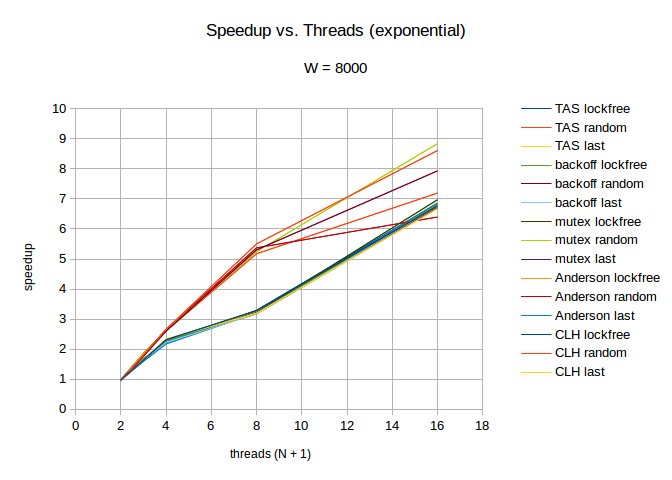
\includegraphics[scale=.8]{packet_3_8000.png}
	\caption{Performance ratios for parallel firewall, with exponential packet distribution at mean work $W = 8000$.}
	\label{packet_3_8000}
\end{center}
\end{figure}

%----------------------------------------------

\begin{figure}
\begin{center}
	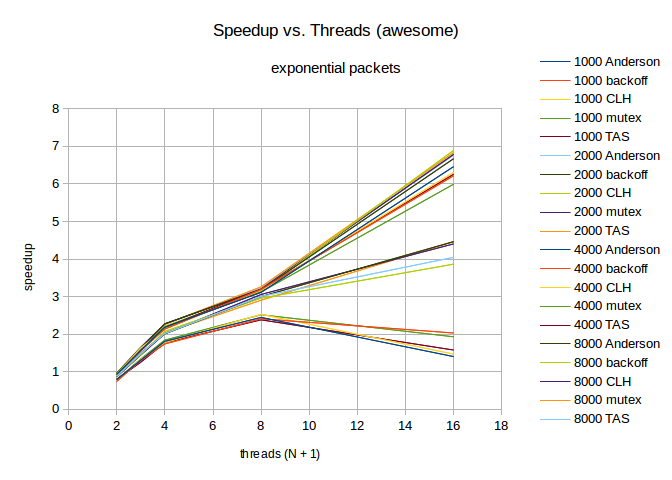
\includegraphics[scale=.8]{packet_4.png}
	\caption{Performance ratios for parallel firewall, with exponential packet distribution and with the awesome scheduling strategy.}
	\label{packet_4}
\end{center}
\end{figure}

\section{Testing}

The crux of the issue here, assuming the firewall was sufficiently tested in the last project, is the ability for each lock to serialize some set of operations. The 
simplest-- and perhaps the most effective-- method for testing this is to spawn $n$ threads making $m$ incrementing calls each on a shared resource, and test to see 
at the end if the shared resource has been altered $n\times m$ times.

\end{document}
